\section{Experimental Results}
In this section, we apply the proposed framework to multiple state-level, daily COVID-19 datasets obtained from the Delphi Epidata API \cite{farrow2015delphi}. These datasets differ in source, structure, and update frequency, and each displays distinct revision patterns, posing challenges for direct performance comparisons across models. Each dataset also exhibits a distinct data revision pattern, making direct comparisons of model performance across datasets nontrivial. 

Beyond evaluating the performance of our proposed method, we compare it against established approaches such as Epinowcast and NobBS in terms of both forecast accuracy and computational efficiency for count-type public health data. We further demonstrate the adaptability of our framework by extending it to weekly datasets, including dengue and ILI case counts. 

All data (including properly versioned datasets) and code used in our analysis are publicly available at:
https://github.com/cmu-delphi/data-revisions-forecasting-paper.

\subsection{Description of Datasets}
\paragraph{Insurance Claims:} We use insurance claims data provided by Change Healthcare (CHNG). CHNG aggregates claim data from numerous healthcare providers and payers, and the information provided by CHNG spans more than two thousand of the most populous US counties, covering more than 45\% of the total US population. Our analysis focuses on a time series comprising the aggregate count of claims featuring ICD codes indicative of COVID-19 diagnoses recorded daily within each county. The reference date corresponds to the claim's date of service, while the report date denotes its appearance in the CHNG database, which may vary considerably depending on providers' claim filing times. Sometimes, Delphi receives the initial report release for a reference date on the same day. We produce forecasts for each report date between 2021-06-01 and 2023-01-10 (a total of 589 days including the Delta wave and the Omicron wave of COVID-19). 

\paragraph{Antigen Tests:}
This dataset is provided by Quidel Corporation (Quidel), which supplies devices used by healthcare providers to conduct COVID-19 antigen tests. We construct a time series of the fraction of positive tests using this dataset. The test records indicate the test date (when the test was conducted) and storage date (when the test was logged into Quidel's MyVirena cloud storage system). The test date serves as the reference date, and test records with a storage date preceding the test date or more than 90 days after are excluded. The report date is defined as the date the records are shared with the Delphi Group via a cloud platform. We produce forecasts for all the states and report dates ranging from 2021-05-18 to 2022-12-12 (a total of 574 days). 

\paragraph{COVID-19 Cases in MA:}
The Massachusetts Department of Public Health (MA-DPH) provides a comprehensive revision history of COVID-19 case reporting\cite{mass_dph_archive}. This dataset includes the 7-day moving average of confirmed COVID-19 cases, updated daily from 2021-01-01, until 2022-07-08. After this date, the reporting frequency transitioned to weekly updates, occurring every Thursday. The first release of the report for a reference date \( t \) is usually made on date \( t+1 \). Unlike the other two datasets—whose fractional denominators exhibit noticeable revision sequences similar to their numerators—a distinctive feature of this dataset is that the COVID-19 confirmed cases are typically normalized by population figures that are sufficiently large to render temporal fluctuations negligible relative to the numerators. We used data reported before 2022-07-08, and produced forecasts for report dates ranging from 2021-07-01, to 2022-06-24 (a span of 359 days).

\subsection{Data Processing}
\paragraph{Data Filtering:}
All datasets are filtered based on the specified time period to ensure data quality. For CHNG outpatient insurance claim data and Quidel antigen test data, this filtering process excludes periods affected by prolonged data reporting issues, such as significant declines in report volume over several months. These anomalies, often manifesting as abrupt shifts in the data distribution, are more indicative of data quality issues than of genuine changes in revision patterns. The MA-DPH case data are filtered to include only the period with consistent daily reporting. As shown in Figure 1, over 90\% of the confirmed cases for a given reference date are reported within 7 days. Given this pattern, developing a data revision forecasting model for weekly reports is unnecessary.

\paragraph{Missing data imputation:}
Before incorporating the data into our framework, we address missing values as defined in the preliminaries. Specifically, for the epidemic count of interest $Y_{it}$ associated with location $i$ and reference date $t$, if $Y_{it}$ has never been reported, impute it as having a historical value of zero. If \( Y_{it} \) is missing for a specific report date \( s \) (i.e., \( Y_{it(s-t)} = \text{NA} \)), we impute it using the most recent available value in the revision sequence of \( Y_{it} \) as of report date \( s \).


\subsection{Experimental Setup}
\begin{figure}[h!]
    \centering
    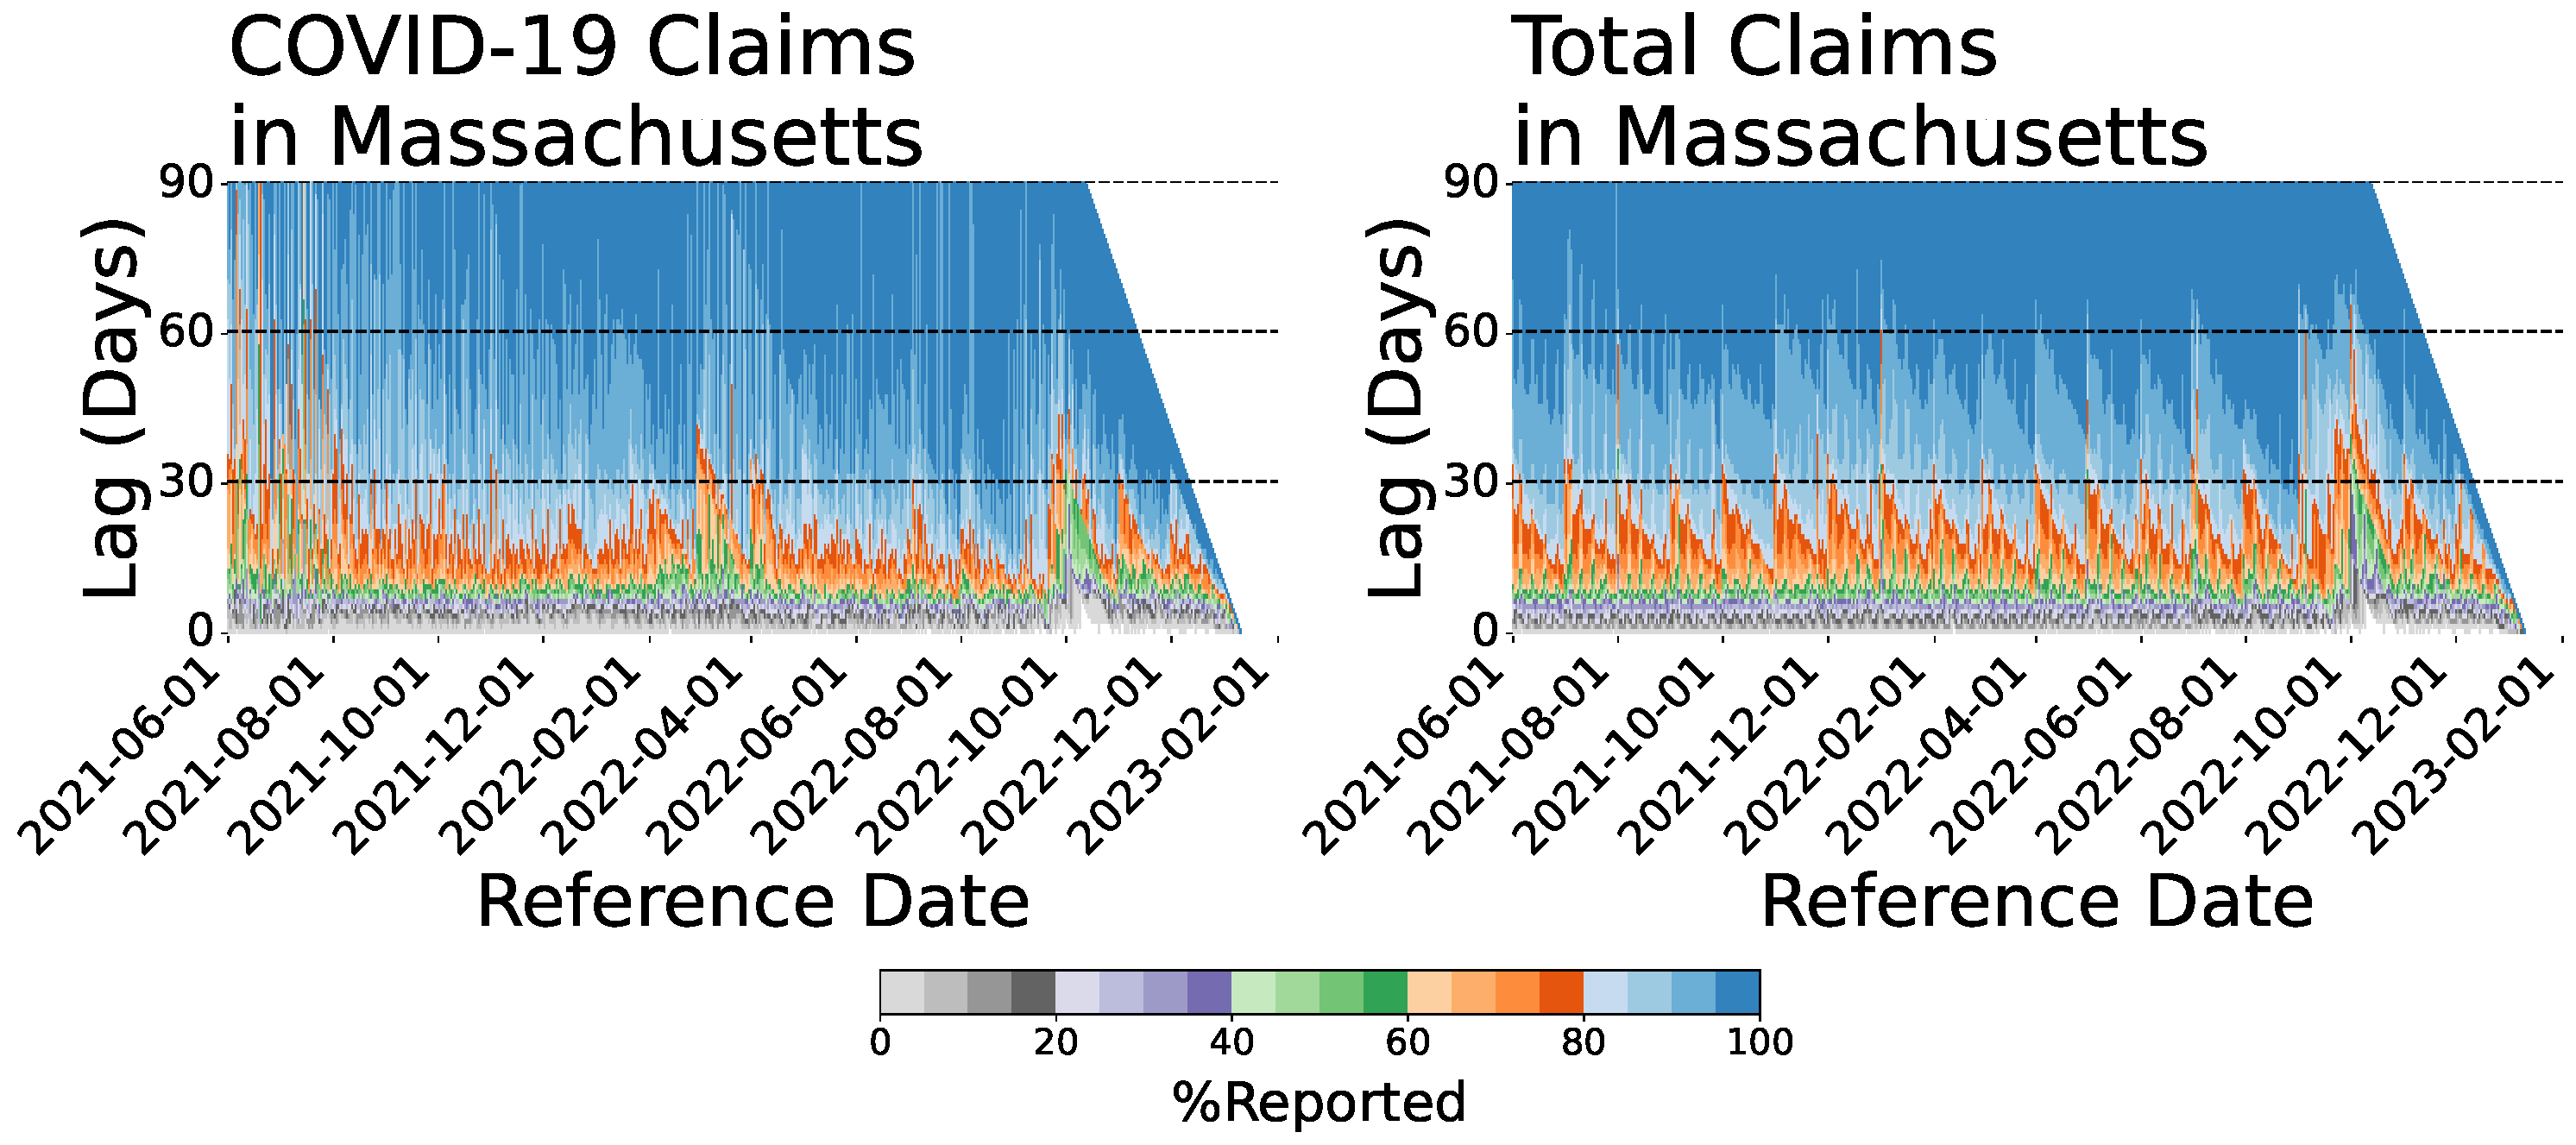
\includegraphics[width=\textwidth]{figs/completeness_Massachusetts.pdf}
    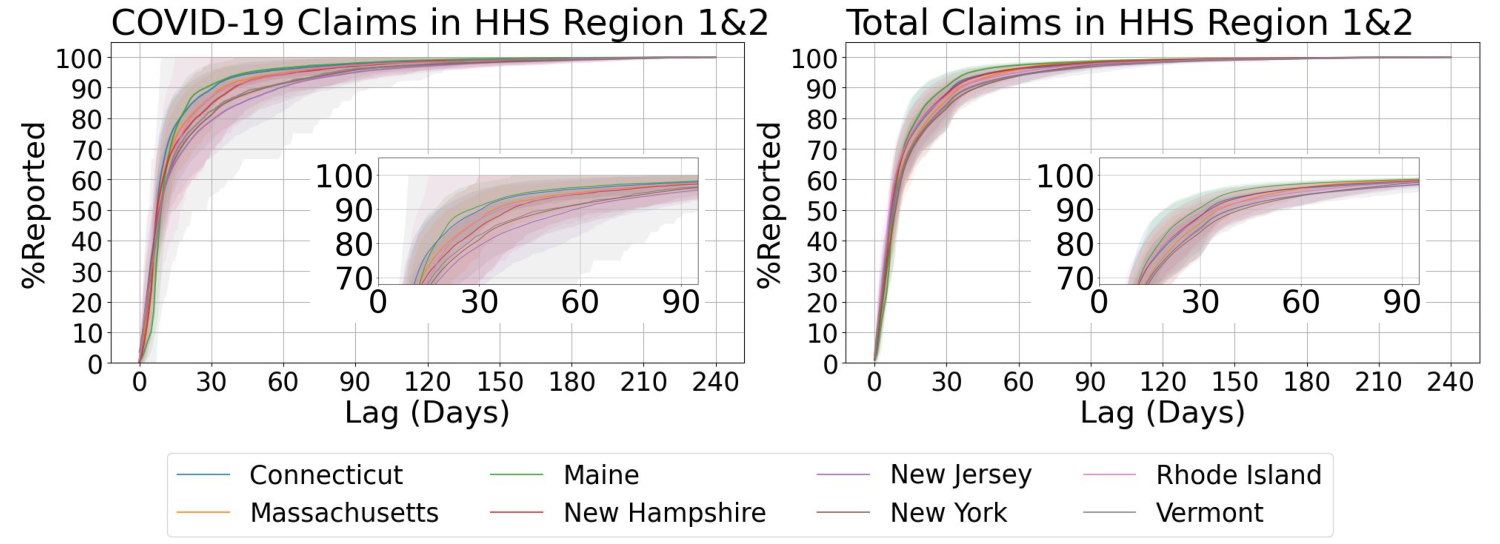
\includegraphics[width=\textwidth]{figs/completeness_lineplot_hhs1&2.pdf}
    \caption{\emph{Top: Distribution of the percentage of reported in Massachusetts, grouped by lag and recorded across reference dates. Bottom: Mean percentage of reported, averaged over all reference dates between 2021-06-01 and 2023-01-10, plotted by lag for states in HHS Regions 1 and 2. Shaded bands represent the 10th to 90th percentile interval. The left panel is based on CHNG outpatient COVID-19 claims data, while the right panel is based on CHNG outpatient total claims data.}}
\end{figure}

\paragraph{Selection of Target Lag $L$:}
To better understand the data revision patterns, we analyze the distribution of the variable \( p_{itl} \), defined as \( p_{itl} = Y_{itl} / Y_{itL_{it}} \), across reporting lags. For count-tyoe data (e.g., the number of confirmed cases), \( p_{itl} \times 100 \% \) quantifies the percentage of the total value reported at the \((l+1)\)th release for location \( i \) and reference date \( t \). For fraction-type data (e.g., the fraction of COVID-19 insurance claims), \( p_{itl} \) represents the normalized provisional estimate. Since the finalized value \( Y_{itL_{it}} \) is not observable in real time, we temporarily approximate it using a sufficiently large lag of 300, under the assumption that the revision process has effectively converged by that point. Specifically, we set $L_{it} = 300, Y_{itL_{it}} = Y_{it,300}$ to serve as a practical surrogate for the finalized target value.


The distribution of $p_{itl}$ provides insight into how data revision sequences evolve over time. In addition to the apparent day-of-week effect and week-of-month effect, the efficiency of data revision is significantly influenced during periods when the epidemic curve is at or near its peak. Figure 2 illustrates this phenomenon using CHNG outpatient insurance claim data in MA as an example. Overall, the revision of COVID-19 claims exhibit greater variance than non-COVID claims, underscoring the difficulty of the forecast task.

Although there may be a considerable degree of heterogeneity in $L_{it}$ (the target horizon for $Y_{it}$, example shown in Figure S1 in Appendix A), the most substantial revisions are typically made within the first two months for the majority locations including states and populous counties for CHNG outpatient insurance claims data. The bottom panel of Figure 2 shows an example based on CHNG outpatient COVID-19 insurance claims data. It reveals that, for states in HHS Region 1 and Region 2, almost all mean \%reported values for COVID-19 reach 90\% when the lag equals 60 days.  

In our experiments, we set \( L = 60 \) for the CHNG outpatient COVID-19 insurance claims data and \( L = 45 \) for the Quidel COVID-19 antigen tests data, both applied uniformly across all states considered. For the data on confirmed cases from MA-DPH, we set \( L = 14 \), ensuring that at least 90\% cases are reported while keeping \( L \) relatively small.

\paragraph{Training Frequency:}
We generate state-level forecasts following the adaptive modeling protocol described in Section 3.2. To improve computational efficiency, model training is performed every 30 days, except for the MA-DPH confirmed case forecasts, where the shorter target lag of 14 days requires retraining every 7 days. While this adjustment reduces computational cost, it may degrade predictive performance in the presence of non-stationarity—particularly in scenarios involving abrupt and substantial changes in data revision patterns—as less frequent retraining limits the model's ability to adapt in a timely manner. On each retraining date \( s_{\text{train}} \), the model is updated with newly available training data and subsequently used to generate quantile forecasts for all epidemic quantities reported on dates \( s \in [s_{\text{train}}, s_{\text{train}}+30) \) (or \( s \in [s_{\text{train}}, s_{\text{train}}+7) \) for the MA-DPH case forecasts).




\paragraph{Location-Specific Model Training:}
Both the CHNG outpatient insurance claims data and Quidel antigen tests data are subject to geographic variation in market share, health-seeking behavior, and reporting practices. These differences render the data incomparable across locations and result in location-specific revision patterns. In this study, we do not attempt to address spatial heterogeneity; instead, we fit the model separately for each location.









